% Documentation du style Latex pour les articles de revues ou de confrences Hermes
% Les consignes aux auteurs sont en annexe de ce document.

\documentclass[fleqn]{article-hermes}
%%% Commandes spcifiques  l'article
%\newcommand{\cfsect}[1]{(\textit{cf.} section~\ref{#1})}
%\newcommand{\cfsectpage}[1]{(\textit{cf.} section~\ref{#1}, page~\pageref{#1})}
%\providecommand{\figureref}[1]{\figname~\ref{#1}}
%\providecommand{\cftab}[1]{(\textit{cf.} tableau~\ref{#1})}
%\newcommand{\cmd}[1]{{\upshape\texttt{\symbol{"5C}#1}}}
%%% Fin des commandes spcifiques  l'article


\journal{\LOBJET. Volume 8 -- n2/2005}{1}{15}

\publisher{03 88 22 21 67 }{00 00 00 00 00}{sonntag@icps.u-strasbg.fr}

\title[Interface Utilisateur Automatique]%
      {Systme expert d'Interface Utilisateur}

\subtitle{Les prmisses de la construction d'interfaces utilisateurs automatique et adaptatif dynamiquement\\  un priphrique}
\author{Maxime Audrin, Jonathan Pont, Sonntag Benoit}

\address{%
ICPS/LSIIT - UMR 7005 - ULP Strasbourg \\
Ple API \\
Bd Sbastien Brant - BP 10413\\
67412 Illkirch CEDEX FRANCE\\[3pt]
maxaudrin@free.fr, jponte@free.fr, sonntag@icps.u-strasbg.fr}

\resume{Le rsum }

\abstract{The abstract }

\motscles{IHM, Interface graphique, langage objet  prototype, Lisaac}

\keywords{IHM, Graphics User Interface, prototype object language, Lisaac}


\begin{document}

%\maketitle % Exemple de 1ere page sans les valeurs de champs
            % pour afficher les commandes  utiliser

\maketitlepage

\section{Introduction et problmatique}
Avec l'volution des technologies, l'informatique a pris une place de
plus en plus importante dans tous les domaines du quotidien :
transports, tlcommunications, appareils electromnagers, mdecine, etc. 
La miniaturisation des composants electroniques a permis l'intgration
de systmes informatiques puissants dans toutes sortes d'appareils. 
La diversit des composants materiels permet egalement de
pouvoir ajouter facilement de nouvelles fonctionnalits que ce soit
par l'ajout de composant matriel ou composant logiciel. 
Si cela permet de rendre de nombreux services dans la vie
courante, la t\^{a}che des concepteurs est loin d'tre simplifie.

\subsection{Adapation des IHMs aux priphriques}
L'informatique embarqu propose une large gamme de
matriel ayant des possibilits diverses et varis en terme de
priphriques d'entres / sorties.
Les interfaces hommes-machines sont fortement li  cette variabilit
de ces priphriques (taille de l'cran, prsence
ou absence de clavier ou de souris, \ldots)
Pour l'informatique de bureau, nous voyons l'mergeance
d'application commune entre diffrent systme d'exploitation et
diffrent support matriel, mais ce mouvement chappe encore 
l'informatique embarqu.
Les plateformes Java intgr dans nos tlphones portables permettent
une abstraction du matriel, mais l'interface utilisateur ne s'adapte
pas au possibilit rel de nos priphriques d'entre / sortie.
Par exemple, les applications prvu pour les {\it{}pocket PC}, voulant
offrir un sous ensemble des possibilit accessible par un ordinateur de
bureau ncessite une reprogrammation complte de leurs IHMs (Exemple\,: 
{\it{}Word pocket}, {\it{}Excel pocket}).

\subsection{Modification des IHMs lors d'ajout de composant logiciel}
Une application devient de plus en plus adaptable via l'insertion
dynamique de {\it{}plugin}. Ces {\it{}plugin} sont des petits
programmes ajoutant des fonctionnalit au sein d'une application.
Ils sont l'quivalent des gestionnaires de priphrique ({\it{}driver})
au niveau logiciel.
L'insertion de ces programmes ont un impact sur l'IHM global d'une
application par l'apparition de nouvelles fonctionnalits.
Trop souvent, le choix des concepteurs est d'ajouter un {\it{}panel}
reprsentant les fonctionnalit de ce {\it{}plugin}. 
Ici, nous soulignons le manque d'intgrit et de la difficult
d'ajouter dynamiquement des fonctionnalits aux sein d'une
application matresse.

\subsection{L'objectifs}
Dans cette article, nous dnonons le caractre trop statique des IHMs
actuelle et la ncessit, de la lourde t\^{a}che, de reprogrammer les
interfaces utilisateurs pour les adapter  un nouveau matriel.

Notre objectif est de librer le concepteur d'une application de la
reprsentation de son interface homme-machine.
Ainsi, l'intrt est que l'IHM d'une application puisse
automatiquement s'adapt  la taille ou type d'cran, aux vnements
matriels ou au type de priphrique d'entres (clavier, cran
tactile, ...). 
Aussi, l'ajout d'une fonctionnalit doit permette une radaptation
automatique et dynamique de IHM envu d'acceuillir de manire le plus
agrable possible cette nouvelle fonctionnalit.

Nos proposons un premier travail de modlisation de cette interface
calcul automatiquement en nous concentrant sur l'infrence d'une IHMs
simplifi dpendant de la taille de l'cran.

Ici nous exposons le plan...


\section{Etat de l'art}
La recherche informatique, dans le domaine de la generation
automatique d'interface graphique, n'en est pas a ses debuts.
En effet, il existait deja des outils connus sous le nom de
User Interface Design Environment comme HUMANOIDE[1],GENIUS[2] permettant
de creer de maniere automatique une interface graphique avec comme contrainte
de fournir des modeles et des schemas graphiques tres complexes.
D'autres outils, plus recents et bases sur le langage XML,
tels que XMLTalks[3], XIML[4], UIML[5], TERASAXML[6], USIXML[7] permettent, eux aussi,
d'atteindre le même but. En ce qui concerne les quatre derniers, on observe une ebauche
"d'adaptation dynamique" mais cela reste exclusivement une specification
a donner au niveau de la creation et ne se fait pas dynamiquement pendant la phase d'execution.
Cependant, tous ces outils permettent surtout de "simplifier" le processus
de creation plutôt que de l'automatiser car il faut y apporter
un nombre d'information assez consequent. De plus, la possibilite
d'adapter dynamiquement cette interface a differents supports
reste exclus. D'autres travaux, plus interessants, peuvent être cites
comme PUC[8](Personal Universal Controller) qui utilise un arbre
de decision ou SUPPLE[9] permettant
une gestion dynamique de l'interface graphique lors d'un changement
de support.\\
Neanmoins, il reste le defaut d'un apport en information encore trop
important et l'incapacite de s'adapter aux possibilites d'entrees/sorties
du peripherique\\
Contrairement a ce qui a ete fait auparavant, nous proposons un mode
de creation d'interface graphique le plus simple possible, sous
forme d'un arbre de fonctionnalite avec une quantite d'element semantique
largement inferieur permettant une automatisation aussi complete 
que possible du processus de conception.
En effet, celle ci se cantonne a trois principales informations par composant de notre interface
que nous detaillerons par la suite.
De plus, elle permet non seulement l'adaptation a la volee de l'interface mais aussi
de prendre en compte la specification du materiel au niveau entrees/sortie.


\section{Les axiomes de notre modele pour le programmeur
  d'application}
Notre modele se base sur la description formelle des fonctionnalites de l'application.
Il s'agit pour le programmeur de construire une structure representant ces fonctionnalites,
munie des informations les caracterisant. Ces informations sont necessaires a l'elaboration d'une interface graphique.

\subsection{Un arbre de fonctionnalite}
Cette structure est representee par un arbre de fonctionnalites de l'application. Les fonctionnalites sont les feuilles de l'arbre et les noeuds sont les etapes par lesquels il faut passer pour acceder a ces fonctionnalites. Ces noeuds seront plus tard modelises par des pattern qui composeront notre interface graphique. Un noeud pourra être un menu, une fenêtre ou autre, et une fonctionnalites un bouton l'activant par exemple (voir paragraphe Description de notre IHM final).\\
Il s'agit pour le programmeur de mettre en commun des fonctionnalites qu'il juge bon de regrouper sous un noeud de l'arbre. Ainsi chaque noeud est une description des noeuds qu'il renferme. Plus on descend en profondeur de l'arbre plus les noeuds gagnent en description. \\
%Regrouper des fonctionnalites sous un noeud permet egalement de ne pas surcharger le noeud pere. En effet moins un noeud 
%comporte de fils, plus facile sera le choix du pattern. Ceci est detaille dans la partie Systeme d'inference.\\
Si nous prenons l'exemple d'une interface traditionnelle, les fonctionnalites permettant l'ecriture/ouverture d'un fichier
(enregistrer, ouvrir, nouveau...) sont disponibles a travers la barre de menus, puis le menu fichier. Nous voyons facilement que la barre de menus est un noeud donnant acces aux menus "Fichier", "Edition" et autres, qui eux-mêmes sont des noeuds donnant acces a d'autres noeuds tels que "Ouvrir" (aboutissant generalement a l'ouverture d'une fenêtre) ou a des fonctionnalites telles que "Enregistrer". Nous pouvons de la même maniere decrire entierement une application: chaque noeud est une description generale des fonctionnalites qu'il renferme et peut donc contenir des fonctionnalites satisfaisant cette description ou mener a d'autres noeuds regroupant des fonctionnalites qui gagnent un degre de precision.\\
La racine de l'arbre est la description generale de l'interface. Seuls ces fils seront affiches sur le peripherique. Il appartient ensuite a l'utilisateur de l'application de faire apparaître les noeuds de profondeur superieure en activant les fils de la racine.\\
Or cet arbre a lui seul ne contient pas d'informations permettant le generation de l'interface graphique.

\subsection{Les ajouts semantiques}
Notre modele prevoit l'ajout d'elements semantiques lors de la construction de l'arbre d'une application. Ceux-ci permettent de decrire d'une part la relation qu'ont entre eux les fils d'un noeud, ce que nous avons appele l'operateur semantique et l'importance d'un noeud dans l'arbre d'autre part, ce que nous avons appele la force d'un noeud.
\subsubsection{L'operateur semantique}
Il y en 3: XOR, OR et AND.\\
L'operateur XOR prevoit que le noeud ne peut pas être actif en même temps qu'un autre: on ne peut pas appuyer sur le bouton "Fichier" et "Edition" en même. C'est un choix exclusif.\\
L'operateur OR a l'inverse permet au noeud de rester active même si l'on active un autre noeud: une check box par exemple.\\
L'operateur AND necessite que l'utilisateur active ce noeud. L'activation de ce noeud est conditionnee par l'activation d'un autre noeud: par exemple, le principe du login et du mot passe. Il faut remplir le champ login et mot de passe avant de pouvoir valider une saisie.
\subsubsection{La force}
C'est un pourcentage qui represente l'importance d'un noeud. Certaines fonctionnalites sont optionnelles et non necessaires au deroulement normal d'une application: ces fonctionnalites, une fois retirees de l'interfaces graphiques (et donc inaccessibles) n'empêchent pas le programme de fonctionner. Notre modele prevoit donc de retirer ces fonctionnalites en dernier recourt afin de proposer une interface graphique plus legere et adequate au peripherique d'affichage.
\subsection{Exemple}
Voici l'arbre abstrait d'une application de dessein.
====>mettre une copie d'écran?
\begin{center}
\includegraphics[scale=0.8]{figures/arbre_abstrait.ps}
\end{center}


\section{Description de notre IHM final}
Une interface graphique est essentiellement composee d'un assemblage de "widget".
Le mot "widget" est la contraction de deux mots venant de l'anglais : "windows" et "gadget".
Ce sont les composants de cette interface qui seront affiche a l'ecran et qui permettront
l'interaction la plus claire et la plus agreable possible entre l'homme et la machine.
Dans le but de respecter l'ergonomie et une certaine convention des interfaces graphiques,
il faut etablir des regles de construction.

\subsection{Composants de base}

Nous pouvons distinguer plusieurs sortes de composants basiques dans notre interface graphique :\\
- Les boutons (button)\\
- Les cases a cocher (check box)\\
- Les boutons radio (radio box)\\
- Le texte (text)\\
- Les icones (icons)\\
- Les raccourcis (shortcut)\\
- Boite d'ecriture (text input)\\
...

D'autres éléments, plus techniques et intrinsèques a la programmation, sont à prendre en compte comme :\\
- La WINOUT : la fenetre principale est une WINOUT et toutes les autres fenetres interne au programme aussi.\\
- La WININ : c'est l'element principal qui compose l'espace de travail (exemple feuille word...)\\

Ce sont toutes ces briques de base qui,une fois compose d'une certaine maniere, aboutiront a la
creation d'elements plus complexes.
%- Button, WIN,...
%- GOUT, GIMG.

\subsection{Composition pour des lments plus complexe}

On peut distinguer plusieurs sortes d'elements former de briques de bases :\\
- La barre de menu : represente un simple assemblage de boutons disposés a l'horizontal\\
- La barre verticale ou horizontal: represente un assemblage de divers éléments de bases comme des boutons, cases a cocher etc..\\
- Le menu vertical : represente un assemblage de boutons disposes a la verticale dans une WINOUT\\
- Le menu horizontal : represente un assemblage de boutons disposes a l'horizontal dans une WINOUT\\
- Le menu deroulant : represente un assemblage de boutons disposes a la vertical dans une WININ\\


\subsection{Axiome de construction}
Il faut pouvoir donner une regle precise lors de la conception de l'interface. Par exemple, un menu horizontal
ne suivra jamais un autre menu horizontal car visuellement parlant, cela nuira a la clarte de l'interface. Une autre 
règle (plus une convention) veut qu'apres une barre de menu ne suivent que des menus verticaux.
Pour veiller a bien respecter ces regles, nous avons élabore une "pseudo-grammaire" representant les axiomes de construction.\\

\begin{center}
\includegraphics[scale=0.8]{figures/grammaire.ps}
\end{center}


\section{Système d'inférence}
Nous avons d'une part un arbre regroupant les fonctionnalités de l'application et contenant les informations nécessaires pour le choix de la modélisation graphique et d'autre part nous avons définit des pattern graphiques potentiellement appliquable à chaque noeud. Nous expliquons ici comment choisir le pattern adéquat en fonction des informations contenues dans l'arbre tout en respectant les spécifications du périphérique d'affichage. Il s'agit deffectuer 2 évaluations pour chaque pattern.
\subsection{Evaluation sémantique}
L'évaluation sémantique d'un pattern doit conclure à sa compatibilité ou non avec ce noeud. Chaque pattern possède sa propre évaluation sémantique. Elle se fait en fonction des caractéristiques propre au pattern et vérifie si le noeud lui-même et ses fils remplisse ces caractéristiques. Par exemple pour remplir les conditions d'un certain patern, un noeud doit posséder un certain opérateur sémantique et ses fils doivent pouvoir être instanciés en tel ou tel pattern. Si c'est le cas on passe à l'évaluation spatiale sinon on teste un autre pattern.
\subsection{Evaluation spatiale}
L'évaluation spatiale vérifie que le pattern respecte les caractéristiques du périphéque d'affichage. Dans un premier temps, nous testons si le pattern ne dépasse pas les limites d'affichage de ce périphérique afin de pouvoir le visualiser en entier. Si c'est le cas nous utilisons le pourcentage représentant la force des noeuds en retirant les fils possèdant une force inférieure à un certain seuil. Nous réitérons cette opération avec des seuils de plus en plus élevés tant que le pattern dépasse les limites du périphérique. Nous exprimons ensuite un pourcentage de recouvrement en fonction du nombre de fils que nous avons retirés.\\
Dans un deuxième temps nous exprimons un pourcentage qui donnera la note finale du pattern pour un noeud. Ce pourcentage est établi en fonction de la surface utilisée par le pattern par rapport à la surface du périphérique d'affichage.
\subsection{Algorithme d'évaluation}
Il s'agit de tester tous les patterns pour chaque noeuds et de garder le meilleur. C'est un problème NP-complet. Nous utilisons pour cela un algorithme récursif. Celui-ci teste chaque pattern sur les fils de la racine et leur évaluation sémantique lance l'évaluation des pattern appropriés sur leurs propres fils. Si au moins un pattern renvoie un pourcentage supérieur à 0 pour chaque fils, alors on passe à l'évaluation spatiale. La récursivité s'arrête aux feuilles. Il s'agit ensuite de garder le meilleur pattern pour chaque noeud en comparant leur note.

\section{Implmentation du modle}

Nous avons choisit d'implémenter notre modele a l'aide du langage Lisaac.

\subsection{Introduction au langage Lisaac}

Lisaac est un langage imperatif a prototype. Il se différencie des langages orientes objet car il ne necessite
ni la creation de classe, ni l'instanciation de l'objet dans le corps du programme. En Lisaac (univers a prototype)
tout est objet (pas de type primitif comme en Java). Un objet n'a pas besoin d'etre instancié, il est "vivant" des le debut
du programme. Ces objets peuvent se cloner et peuvent posseder plusieurs parents à n'im- La barre d'outils : represente un assemblage de divers éléments de bases comme des boutons, cases a cocher etc..\\porte quel moment de la vie
du programme (multi-heritage dynamique).

\subsection{Reprsentation par hritage dynamique de l'arbre}

Chaque noeud de notre arbre est represente par un prototype appele "group" ayant un lien 
d'heritage statique avec un prototype "groupref". Dans ce dernier, sont regroupees toutes les caracteristiques
necessaires du noeud.
Chaque pattern est représenté par un prototype possédant chacun une méthode d'évaluation sémantique et spatiale, et hérite du prototype groupref. Ce prototype contient uniquement des méthodes défférées (abstraites) qui sont définies dans les prototypes des pattern. En effet nous changeons dynamiquement le parent d'un noeud (prototype group) pour le faire hériter d'un pattern et ainsi pouvoir utiliser ses propres fonctions d'évaluation. C'est l'héritage en losange. Il permet au prototype group de connaitre à la compilation les méthodes qui seront utilisées après un héritage dynamique vers un pattern.
Ce type d'héritage est illustré sur le schéma ci-dessous.

%\begin{figure}
\begin{center}
\includegraphics[scale=1.0]{figures/GUII.ps}
%\caption{Arbre héritage dynamique}
%\label{tree_dynamic}
\end{center}
%\end{figure}

\section{Rsultat}

\section{Travaux futurs}

\section{Conclusion}


\end{document}
